\chapter{Outline of the project}
\label{chap:outline}

\section{Objectives}
\subsection{Primary objectives}
The goal is to build a software system, using computer vision algorithms. First of all, it should be able to estimate the frame-to-frame motion of a racing car and the momentary orientation of the camera with respect to the ground plane. Secondly, at any time, the system should be able to create a birds eye view map of the environment that is in front of the car, in particular the positions of the cones which are used to mark the drivable path.\bigskip 

\subsection{Secondary objectives}
When a good solution is found to these two problems, the system could be expanded and obstacles, side barriers etc. could be entered into the map previously mentioned. Based on the previous features of the system, two additional features could be added: reconstruction of the car's trajectory over time and building a global map from the instantaneous map.\bigskip

These last two additional features are a nice addition to the primal goals, but will only be investigated once the primal goals are working properly.\bigskip

\section{The motion model}
When we talk about motion, we have to define how this motion will be described. Equally important is to define the coordinate frames we will be working with.

\subsection{Motion parameters}
Every 3-D rigid motion can be decomposed into three components. A motion is always happening in a certain plane, to define this plane uniquely, the normal vector $\vt$ is used. The displacement in this plane is called the translation and can be expressed by the translation vector $\vt$. The third parameter is the rotation, this can be expressed with the rotation matrix $\MR$.\bigskip

A 3-D rotation always consists of three components, a yaw, a pitch and a roll. These parameters will be discussed more thoroughly in section \autoref{ssec:rotmat}.

\subsection{Coordinate frames}
We are working with camera images, which are 2-D representations of points in a 3-D world. It is thus of utmost importance to define the coordinate frames we will be using to avoid confusion.\bigskip

First of all, there is the image itself. This is a 2-D frame with x-axis and y-axis along the horizontal axis and vertical axis of the image respectively. The unit of these coordinates is measured in pixels and the center of the frame is at the top left of the image.\textbf{ADD FIGURE}\bigskip

Secondly, there is the camera coordinate system, which we will also use for the car as the camera is rigidly attached to the car. This is a right-handed 3-D coordinate system. The center of the frame is located at the center of the camera (model). The x-axis is pointing left, the y-axis is pointing up and the z-axis is leaving the camera perpendicular to the camera in the direction of the view. \textbf{ADD FIGURE}\bigskip

The third and last coordinate frame is the real world system. This is also a right-handed 3-D coordinate system and to keep things simple, this can be defined as the camera coordinate system at frame 1.\bigskip

As we are working with three different coordinate frames, it's important to know how to transfer points from one frame to another. We'll discuss this at length in a later section.

\subsection{Motion equation}
We have talked about motion and the motion parameters. Each frame-to-frame motion will be described using these parameters in a motion equation.\bigskip

To define this equation, take two points in the real world frame: $P_1 = (X_1, Y_1, Z_1)^T$ and $P_2 = (X_2, Y_2, Z_2)^T$. The transformation from $P_1$ to $P_2$ can be described as follows:
\begin{equation}\label{eq:motion}
    \begin{pmatrix}
        X_2 \\ Y_2 \\ Z_2
    \end{pmatrix} =  \MR \begin{pmatrix}
        X_1 \\ Y_1 \\ Z_1
    \end{pmatrix}+ \vt
\end{equation}

\subsubsection{Homogeneous coordinates}
In what follows, we'll use Homogeneous coordinates instead of Cartesian coordinates. The use of Homogeneous coordinates makes some formulas easier to work with and lets us represent projective transformations by a matrix. \bigskip

To write the motion equation from \autoref{eq:motion} in Homogeneous coordinates, we take $P_1 = (X_1, Y_1, Z_1, 1)^T$ and $P_2 = (X_2, Y_2, Z_2, 1)^T$ and come to the following equation:
\begin{equation}
    \begin{pmatrix}
        X_2 \\ Y_2 \\ Z_2 \\ 1
    \end{pmatrix} = \begin{pmatrix}
        \MR & 0 \\
        0 & 0
    \end{pmatrix} \begin{pmatrix}
        X_1 \\ Y_1 \\ Z_1 \\ 1
    \end{pmatrix} + \begin{pmatrix}
        t_1 \\ t_2 \\ t_3 \\ 1
    \end{pmatrix}
\end{equation}
which can be rewritten as
\begin{equation}
    \begin{pmatrix}
        X_2 \\ Y_2 \\ Z_2 \\ 1
    \end{pmatrix} = \begin{pmatrix}
        \MR & \vt \\
        0 & 1
    \end{pmatrix} \begin{pmatrix}
        X_1 \\ Y_1 \\ Z_1 \\ 1
    \end{pmatrix}
\end{equation}
This matrix characterises the transformation or motion that occurred between two frames. Based on these transformation matrices, the position of the camera (and thus the car) can be determined by concatenating the transformations.

\subsection{Rotation matrix}\label{ssec:rotmat}
We have mentioned the rotation matrix $\MR$, but thus far it is not clear what this actually means. A rotation can always be decomposed in three components: yaw, pitch and roll. \bigskip
\begin{figure}
    \centering
    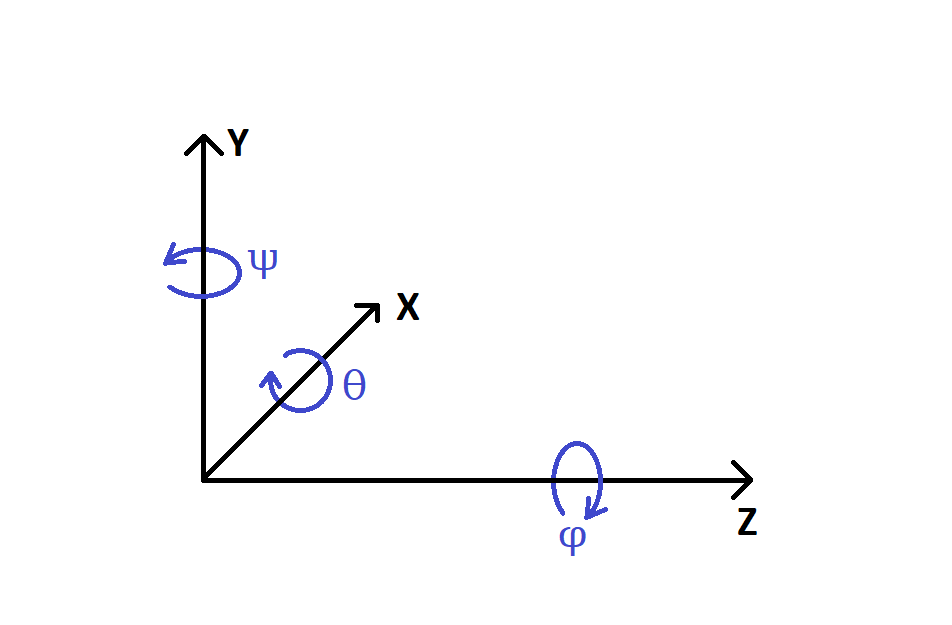
\includegraphics[width=1\textwidth]{figures/yaw_pitch_roll.png}
    \caption{Yaw, pitch and roll}
    \label{fig:rotations}
\end{figure}

\autoref{fig:rotations} shows these rotation components. $\psi$, $\theta$ and $\phi$ are yaw, pitch and roll respectively. As it is a right handed system, we have the following conventions:
\begin{itemize}
    \item When $\psi$ is positive, there is a rotation to the left.
    \item When $\theta$ is positive, there is an upward rotation.
    \item When $\phi$ is positive, there is a clockwise rotation.
\end{itemize}
This is all when looking forward from the center alongside the Z-axis.\bigskip

Each of these rotation components can be defined by a $3\times3$ matrix:
\begin{equation}
    \MR_y(\psi) = \begin{pmatrix}
        \cos\psi & 0 & \sin\psi \\
        0 & 1 & 0 \\
        -\sin\psi & 0 & \cos\psi
    \end{pmatrix}
\end{equation}
\begin{equation}
    \MR_x(\theta) = \begin{pmatrix}
        1 & 0 & 0 \\
        0 & \cos\theta & -\sin\theta \\
        0 & \sin\theta & \cos\theta \\
    \end{pmatrix}
\end{equation}
\begin{equation}
    \MR_z(\phi) = \begin{pmatrix}
        \cos\phi & -\sin\phi & 0 \\
        \sin\phi & \cos\phi & 0 \\
        0 & 0 & 1
    \end{pmatrix}
\end{equation}
To get the rotation matrix $\MR$, we multiply the yawn, pitch and roll like this:
\begin{equation}
    \MR = \MR_z(\phi)\cdot\MR_y(\psi)\cdot\MR_x(\theta)
\end{equation}
\begin{equation*}
    = \begin{pmatrix}
    \cos\psi\cos\phi & \sin\theta\sin\psi\cos\phi - \cos\theta\sin\phi & \cos\theta\sin\psi\cos\phi + \sin\theta\sin\phi \\
    \cos\psi\sin\phi & \sin\theta\sin\psi\sin\phi + \cos\theta\cos\phi & \cos\theta\sin\psi\sin\phi - \sin\theta\cos\phi \\
    -\sin\psi          & \sin\theta\cos\psi                                  & \cos\theta\cos\psi \\
  \end{pmatrix} 
\end{equation*}

\section{Determining motion}\label{sec:determmot}
We now have a way to describe motion in the form of a rotation matrix and a translation vector. To determine this motion, we need to have some corresponding points from each pose. Assuming we have these (we'll discuss in detail later how to get these) there are two cases, the general case where the keypoints can not all lie in one plane. However if this is the case, there's a second option to handle this. The difficulty in all this is that we are working with images, which are 2-D representations of a 3-D world. 

\subsection{General case: points not in one plane}
In general, we have a perspective model because we work with a camera that can be simplified to the pinhole camera model. The equations that relate motion to the image coordinates are non-linear in the motion parameters \cite{tekalp}. A two-step linear algorithm was developed in order to get the motion parameters from (at least eight) point correspondences. Doing this, an intermediate essential matrix $\ME$, consisting of the so called essential parameters is estimated. The way this algorithm works will be discussed in detail later on.

\subsubsection{Essential matrix}
The essential matrix encodes the epipolar geometry of two images. Thus, to break down the essential matrix, we need to have a look at epipolar geometry. \autoref{fig:epigeo} shows a camera in two positions $O_L$ and $O_R$. Point $X$ is projected onto the left image plane resulting in $X_L$ and onto the right image plain resulting in $X_R$.\bigskip

The points $e_L$ and $e_R$ are called the epipoles or epipolar points. They are the projection of the other camera position (its perspective center) onto the image plane. They lay on one line together with the perspective centers $O_L$ and $O_R$.\bigskip

From the perspective of $O_L$, the line $X-O_L$ is a single point $X_L$ while from the perspective of $O_R$ this is a line. This line $e_R-X_R$, shown as a red line in \autoref{fig:epigeo} is called an epipolar line.\bigskip

When the projection $X_L$ onto the left image plane is known as well as the epipolar line $e_R-X_R$ and point $X$ is projected onto the right image plane: $X_R$ evidently laying on the epipolar line, then each point observed in one image must be observed in the other image on a known epipolar line. This gives us an epipolar constraint, that for each set of points it is possible to test whether they correspond to the same 3-D point. This epipolar constraint can be described by an essential matrix.\bigskip

The essential matrix maps a point in one image to an epipolar line in the other image. If you take a point in one image and multiply it by the essential matrix, you will get the epipolar line on the other image. This essential matrix can then be decomposed into the rotation matrix and translation vector, in \autoref{ssec:essentialmat} we will discuss in detail how to estimate and then decompose the essential matrix.

\begin{figure}
    \centering
    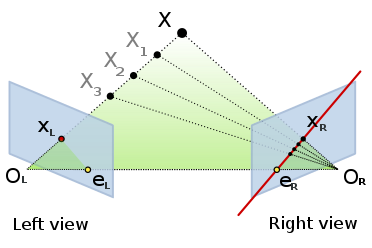
\includegraphics[width=1\textwidth]{figures/epipolar_geometry.png}
    \caption{Epipolar geometry}
    \label{fig:epigeo}
\end{figure}

\subsection{Special case: points in one plane}
When all points lay in one plane, the general case with the essential matrix does not belong to the possibilities. Fortunately, there is another way to deal with this case. To do this, we introduce the term Homography. \bigskip

A homography relates the transformation between two planes up to a scaling factor. We will discuss the scale ambiguity later. A homography matrix is a $3\times3$ matrix with 8 degrees of freedom as we have an unknown scale factor.\bigskip

If we have a planar surface $P = (x, y, 1)^T$, then after transforming this plane (by e.g. changing the camera angle) it will be transformed to $P' = (x', y', 1)^T$. The transformation from $P$ to $P'$ can be expressed using the homography matrix like this:
\begin{equation}
    s\begin{pmatrix}
        x' \\ y' \\ 1
    \end{pmatrix} = \MH \begin{pmatrix}
        x \\ y \\ 1
    \end{pmatrix}
\end{equation}
$s$ being the unknown scale factor. Note that we are using homogeneous coordinates instead of euclidean coordinates.\bigskip

It is clear that it is possible to estimate a homography matrix if we have multiple corresponding points on both planar surfaces. This homography can then be decomposed into the rotation matrix, translation vector and normal vector. How to estimate the homography and how to decompose it will be discussed in detail later on.

\subsection{Combining both}
Using one of these does not have to exclude using the other. As the footage we will be using will have both points laying on a fixed planar surface (being the road surface) and points spread out in space, we can use the essential matrix and homography matrix complementary.

\section{Point-to-point correspondences}
In \autoref{sec:determmot} we talked about the need for point correspondences in consecutive frames to estimate either the essential or homography matrix in order to determine motion.\bigskip

\subsection{Local image features}
To look for point correspondences, we first need to look for recognisable points. A local image feature describes a small region of an image. It consists of a keypoint, which is the image coordinate of the image patch and a descriptor which describes the content of that patch.\bigskip

Using a keypoint detector it is possible to find keypoints in an image. Keypoint description methods make it possible to describe the patch and compare keypoints across different images. In section \autoref{sec:keydet} we describe these in detail as well as the used keypoint detector and description methods.